\documentclass[aspectratio=169,compress]{beamer}
\pdfpagewidth\paperwidth
\pdfpageheight\paperheight
\usepackage[greek,italian]{babel}
\usepackage[utf8x]{inputenc}
\usepackage[T1]{fontenc}
\usepackage{lmodern,amsmath,amssymb,tipa,cclicenses,graphicx,subcaption,adjustbox}

\usetheme[background=light]{metropolis}%numbering=none
\useoutertheme{split}
\hypersetup{pdfstartview={Fit}} % fits the presentation to the window when first displayed

\metroset{block=fill}

\begin{document}
\title{Corso introduttivo a \LaTeX}
\subtitle{Lezione 1}
\author{Davide Peressoni}
\institute[]{Commissione Informatica\\Collegio Universitario don Nicola Mazza}
\date%[DATE CURTE]
{28 Novembre 2018}
\titlegraphic{
\includegraphics[height=80px]{ComInfo}}

\setbeamertemplate{title page}{
  \begin{minipage}[b][\paperheight]{\textwidth}
    \vfill%
    \ifx\inserttitle\@empty\else\usebeamertemplate*{title}\fi
    \ifx\insertsubtitle\@empty\else\usebeamertemplate*{subtitle}\fi
    \usebeamertemplate*{title separator}
    \vspace*{1cm}
    \adjustbox{valign=M}{\ifx\inserttitlegraphic\@empty\else\usebeamertemplate*{title graphic}\fi}
    \adjustbox{valign=M}{\begin{minipage}{200px}
      \ifx\beamer@shortauthor\@empty\else\usebeamertemplate*{author}\fi
      \ifx\insertdate\@empty\else\usebeamertemplate*{date}\fi
      \ifx\insertinstitute\@empty\else\usebeamertemplate*{institute}\fi
    \end{minipage}}
    \vfill
    \vspace*{1mm}
  \end{minipage}
}
\setbeamertemplate{title graphic}{\inserttitlegraphic}

\maketitle

  
% \frame{\transfade
%   \frametitle{Table of Contents}
%   \tableofcontents[hideallsubsections]
% }
\frame{
  \tiny\cc 2018 Davide Peressoni\\~\par
    \emph{Le informazioni contenute nel presente docuemnto sono state verificate e documentate con la massima cura possibile. Nessuna responsabilità derivante dal loro utilizzo potrà venire imputata all’Autore coinvolto nella loro creazione, pubblicazione e distribuzione.}\\~\par
    Alcuni diritti riservati.\\~\\
    Documento prodotto con \LaTeX.\\
    Questo documento è rilasciato con licenza\\
    \begin{figure}[!ht]
	\centering
	    
\includegraphics{../Lezione1/CC.pdf}
    \end{figure}~\\
    \textbf{Creative Commons BY-NC-SA 4.0}\\
    Attribuzione – Non Commerciale - Stessa licenza\\
    \url{http://creativecommons.org/licenses/by-nc-sa/4.0/}\\
    \textbf{Attribuzione} — Devi riconoscere una menzione di paternità adeguata, fornire un link alla licenza e indicare se sono state effettuate delle modifiche. Puoi
    fare ciò in qualsiasi maniera ragionevole possibile, ma non con modalità tali da suggerire che il licenziante avalli te o il tuo utilizzo del materiale.\\
    \textbf{Non commerciale} — Non puoi usare il materiale per scopi commerciali.\\
    \textbf{Stessa licenza} — Se remixi, trasformi il materiale o ti basi su di esso, devi distribuire i tuoi contributi con la stessa licenza del materiale originario.
}

\section{Cos'\`{e} \LaTeX?}
\frame{\transfade\centering
\LaTeX{} \only<2>{(/\textipa{"la:tEx}/,[\textipa{"latek}]; dal greco \begin{otherlanguage}{greek}τέχνη\end{otherlanguage})}\only<3->{è un linguaggio di markup.}
\only<4->{\\~\\Descrivere il documento}
\only<5->{\begin{figure}
  \captionsetup[subfigure]{labelformat=empty}
  \centering
  \begin{subfigure}[b]{0.4\textwidth}
      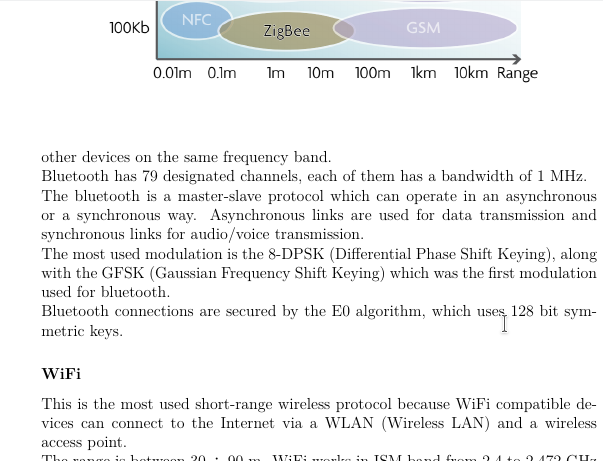
\includegraphics[width=\textwidth]{img/writer}
      \caption{Writer}
  \end{subfigure}~
  \visible<6->{\begin{subfigure}[b]{0.4\textwidth}
      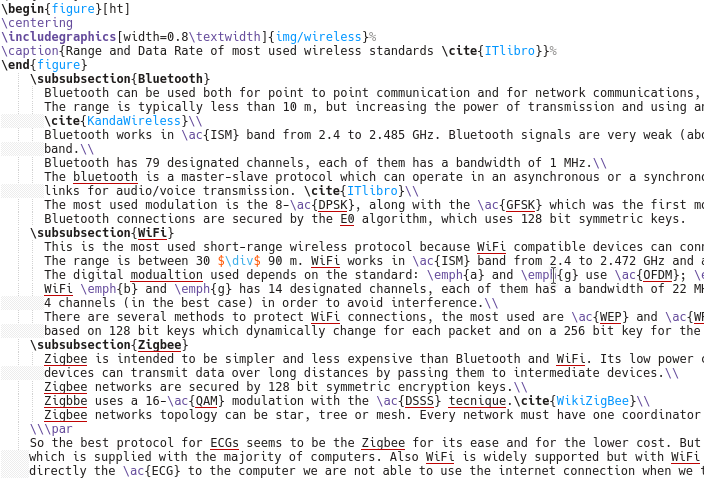
\includegraphics[width=\textwidth]{img/latex_source}
      \caption{Latex}
  \end{subfigure}}
\end{figure}}
}

\frame{\transfade\centering
\frametitle{I vantaggi di \LaTeX}
\begin{itemize}
\item<2-> i documenti hanno un'impaginazione perfetta e risultano piacevoli alla lettura
\item<3-> con un po' di esercizio di possono comporre formule matematiche, schemi a blocchi, circuiti,\dots{} semplicemente
\item<4-> la formattazione non subirà mai modifiche drastiche e risulterà uniforme
\end{itemize}
}

\frame{\transfade\centering
\frametitle{Cosa si può fare con \LaTeX?}
\only<1>{
  \begin{columns}\begin{column}{0.4\textwidth}\centering
  Articoli, Relazioni, Libri, Lettere,~\dots
  \end{column}\begin{column}{0.6\textwidth}
  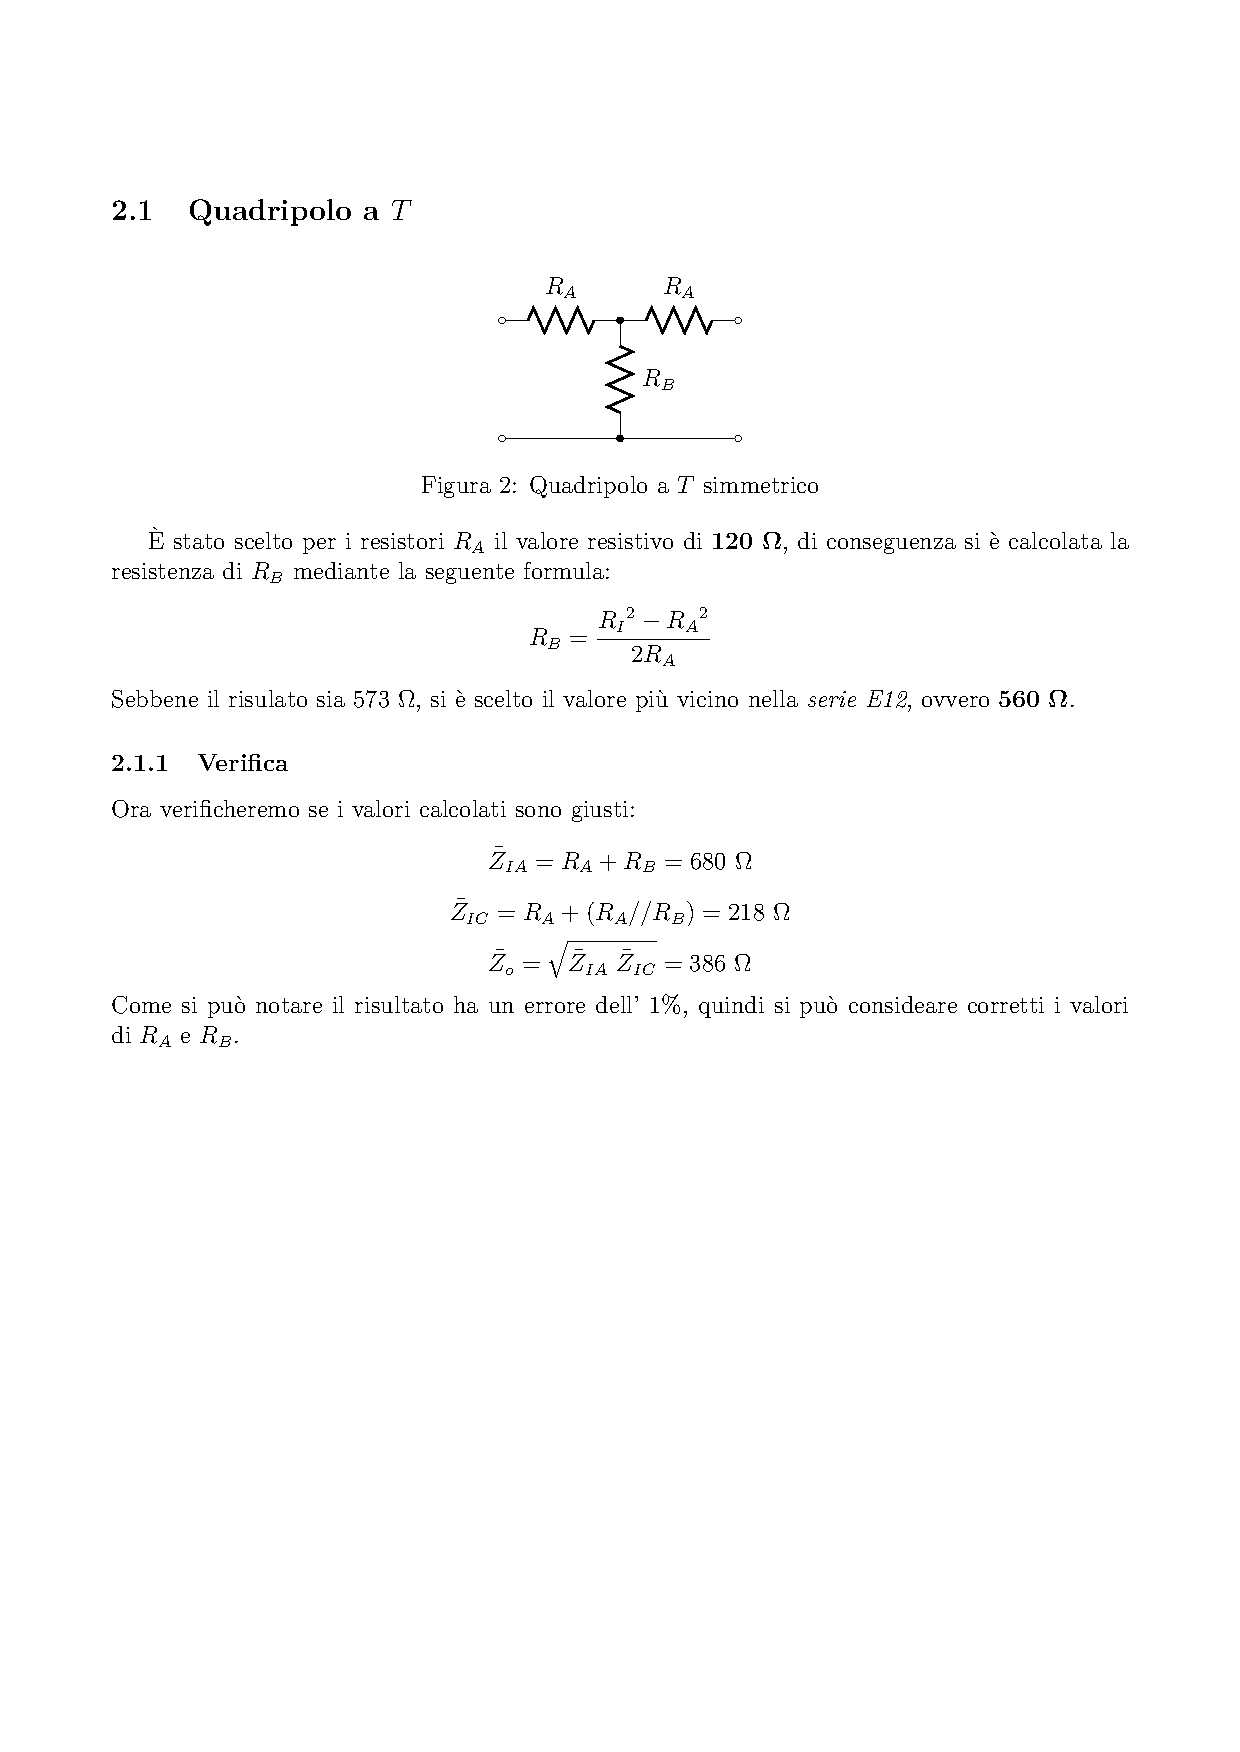
\includegraphics[height=0.8\textheight]{img/relazione}
  \end{column}\end{columns}
}
\only<2>{
  Circuiti, Schemi, Tabelle, Grafici,~\dots\\
  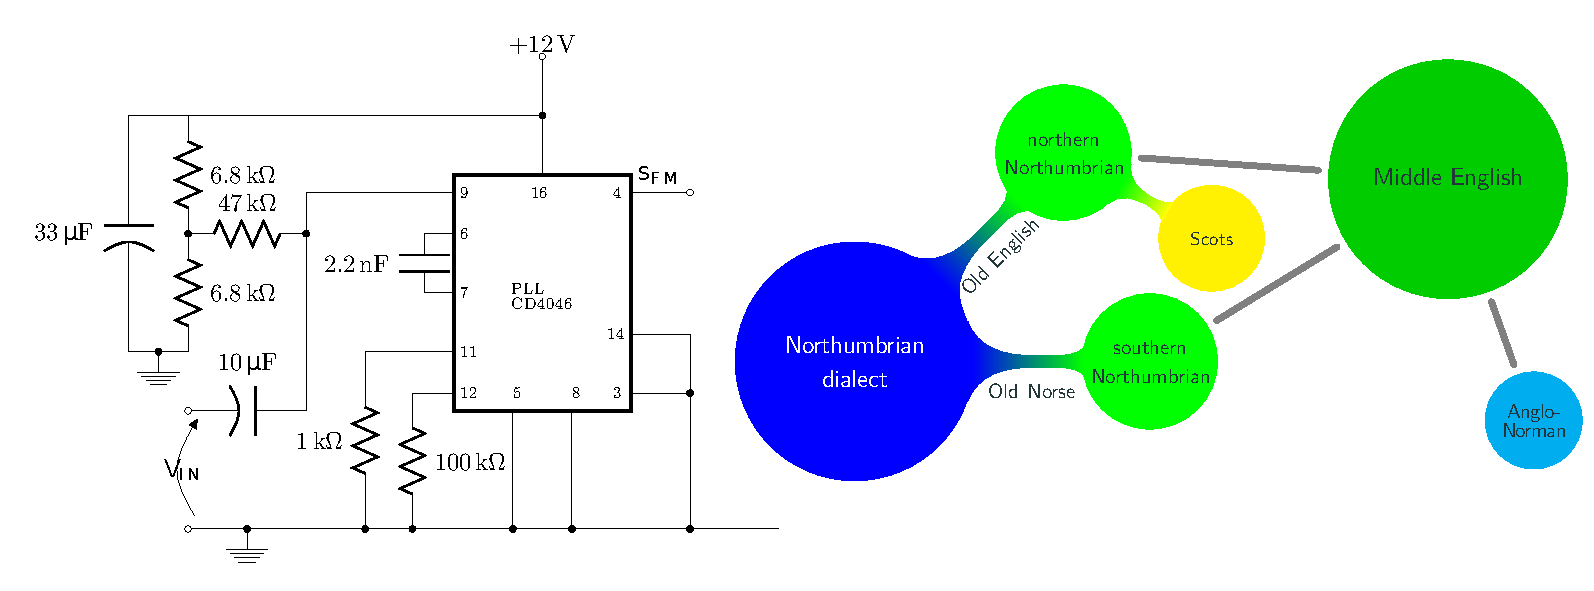
\includegraphics[width=0.9\textwidth]{img/schemi}
}
\only<3>{
  Formule chimiche\\
  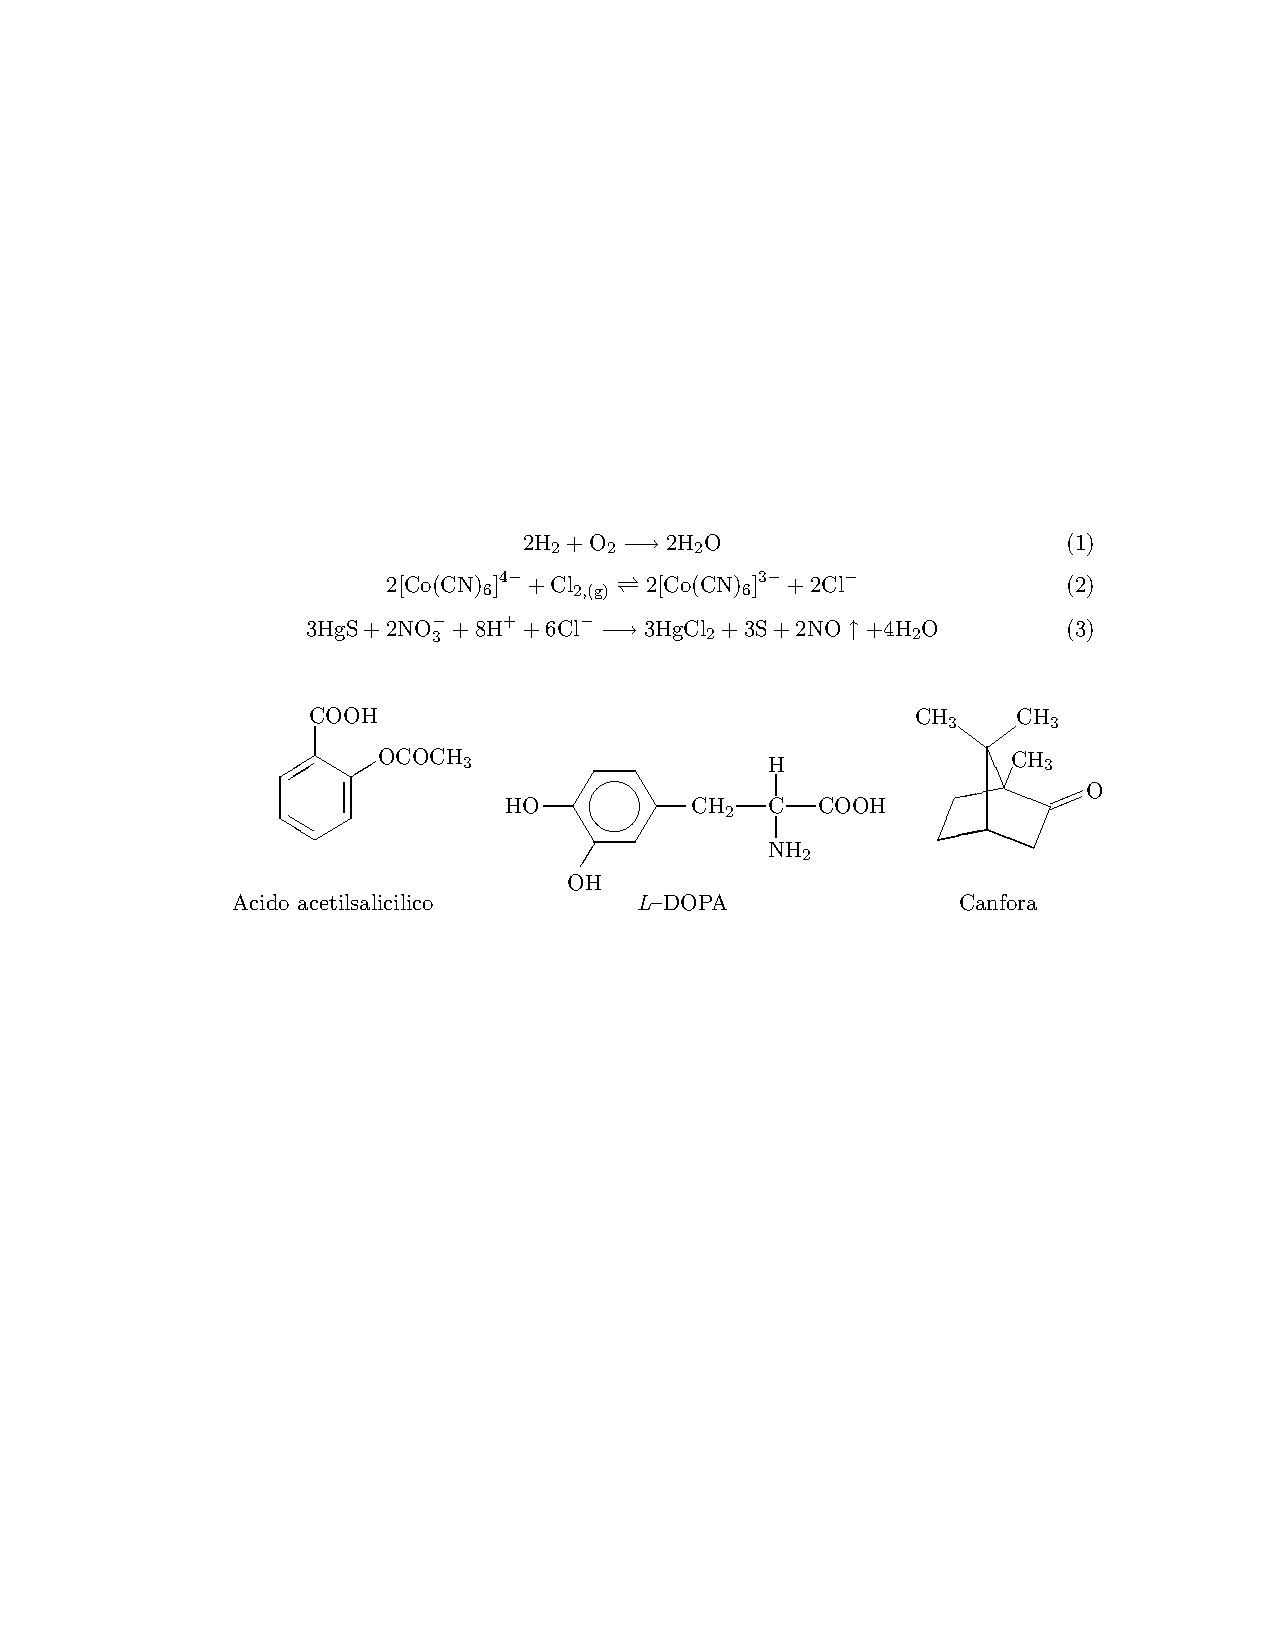
\includegraphics[width=0.9\textwidth]{img/chimica}
}
\only<4>{
  Accordi, Spartiti,~\dots\\
  \begin{figure}
    \captionsetup[subfigure]{labelformat=empty}
    \centering
    \begin{subfigure}[b]{0.4\textwidth}
        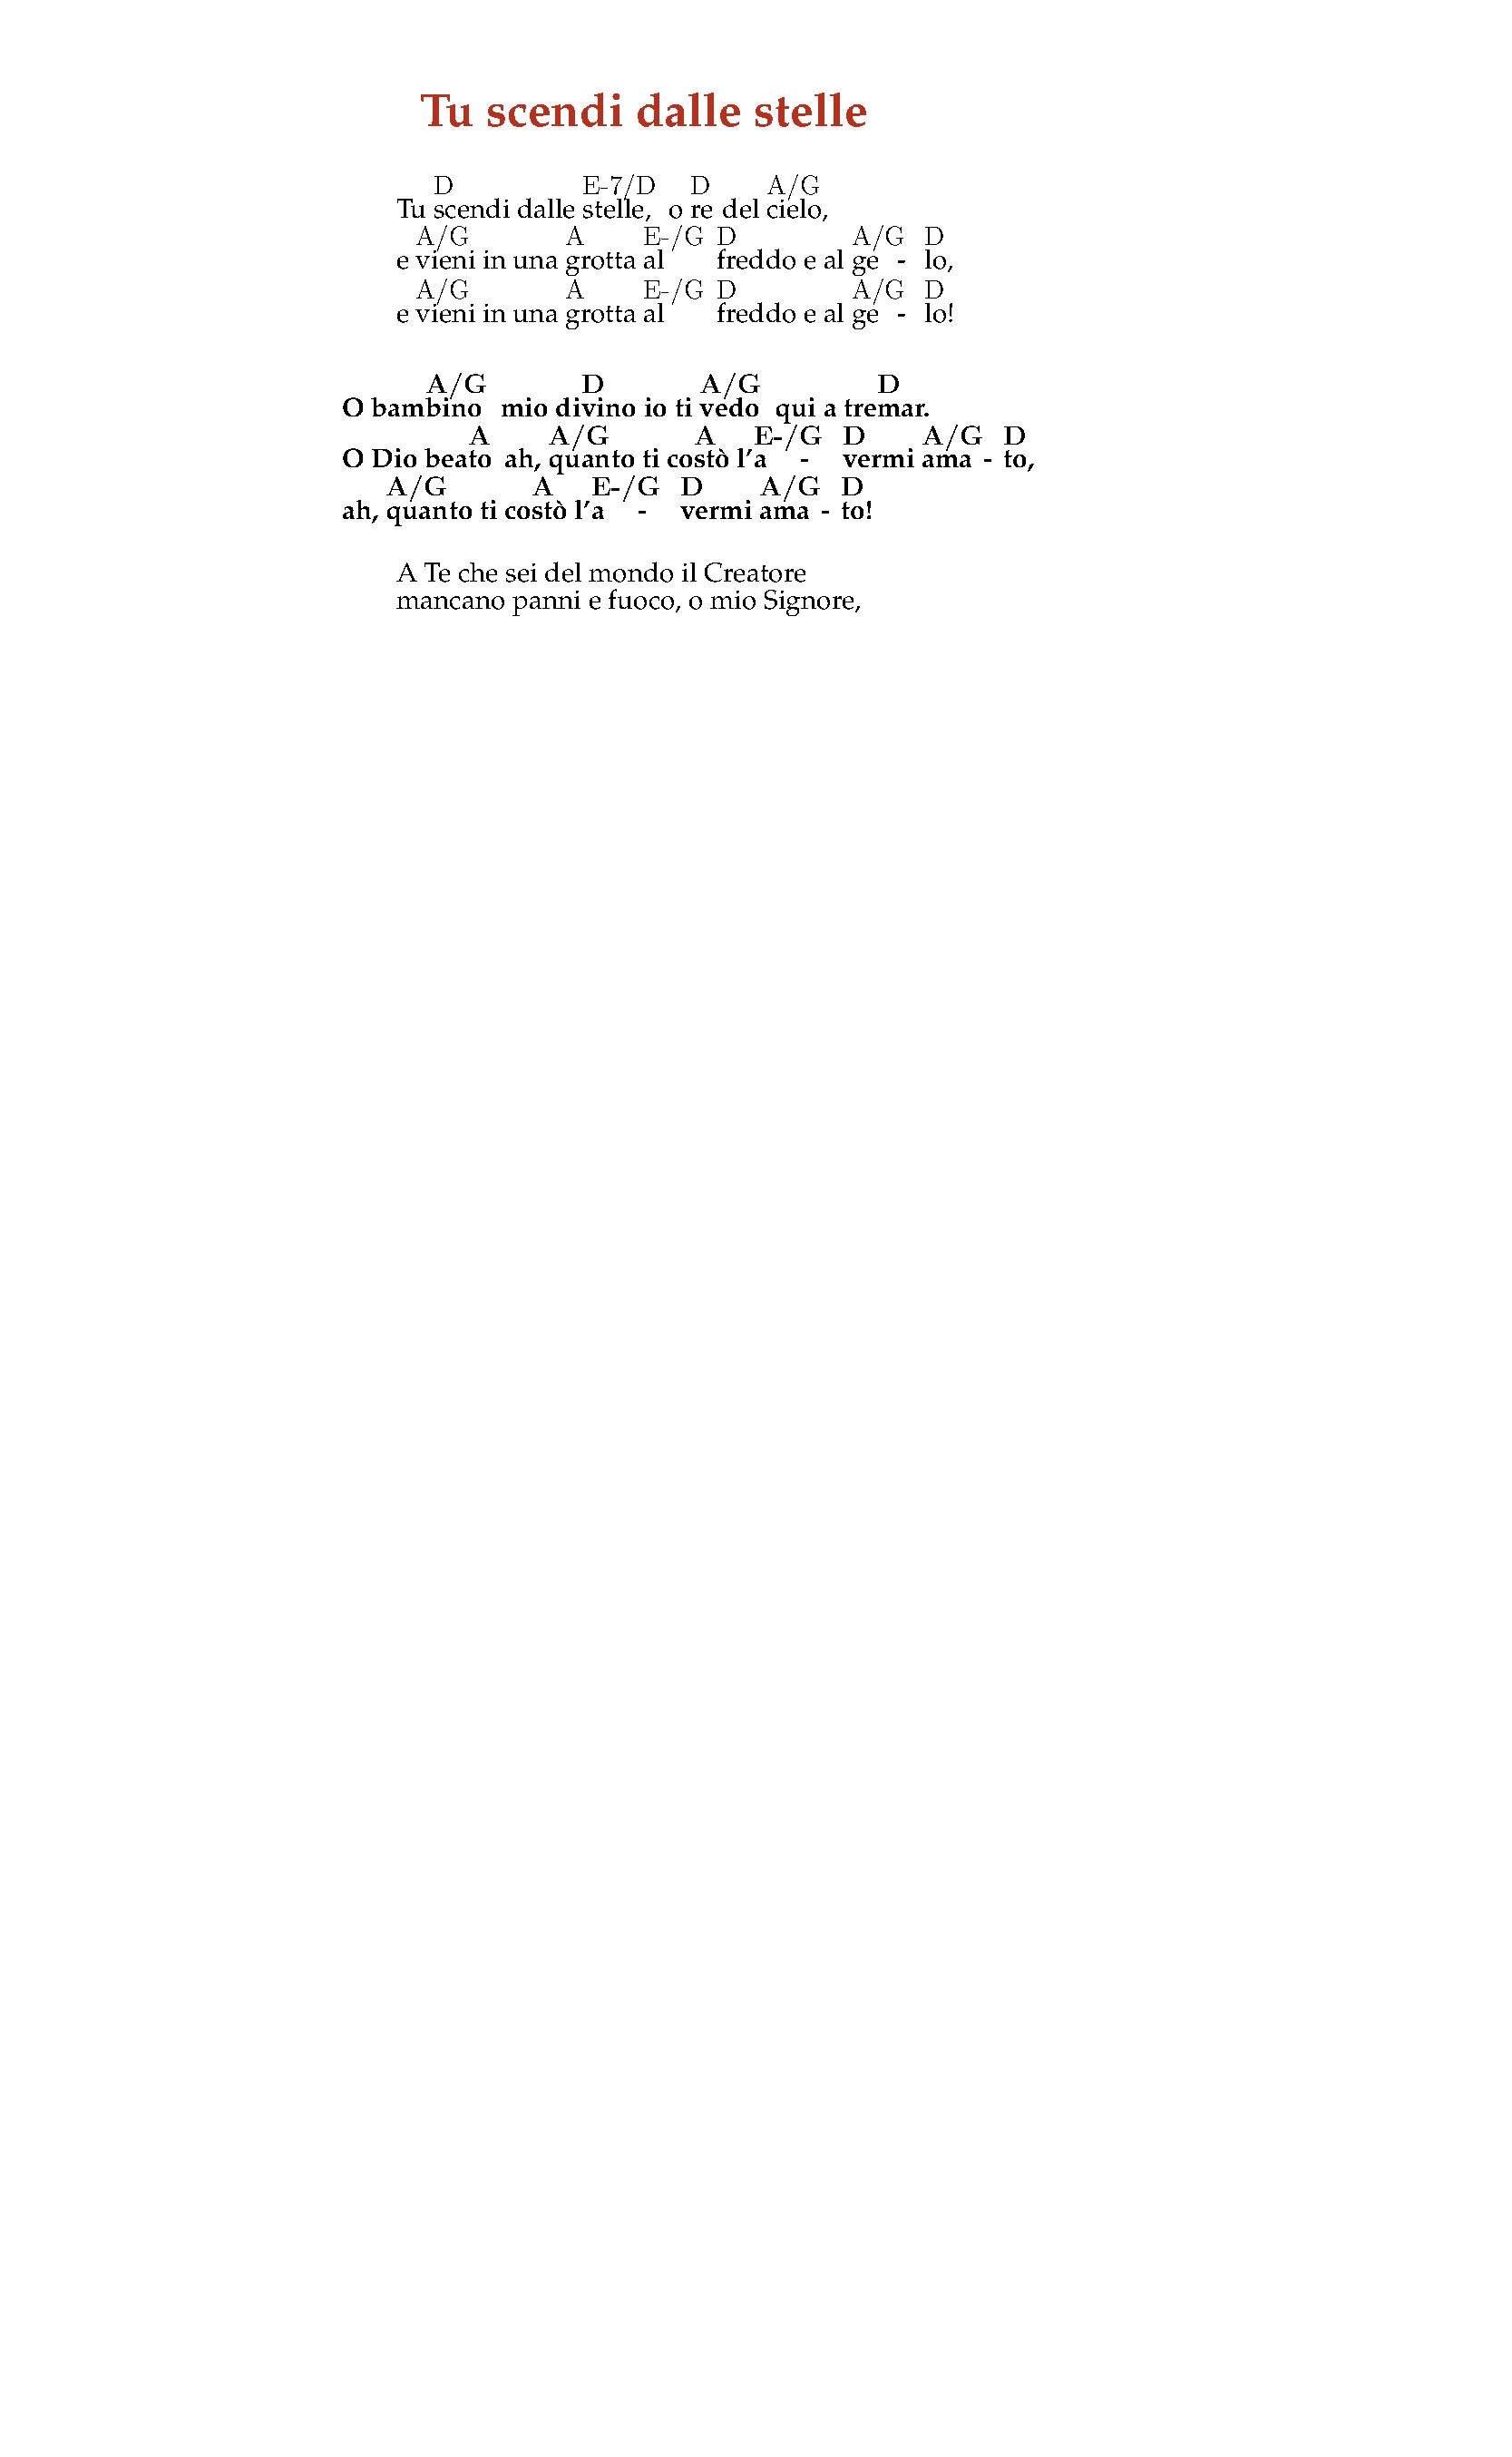
\includegraphics[width=\textwidth]{img/accordi}
    \end{subfigure}~
    \begin{subfigure}[b]{0.6\textwidth}
        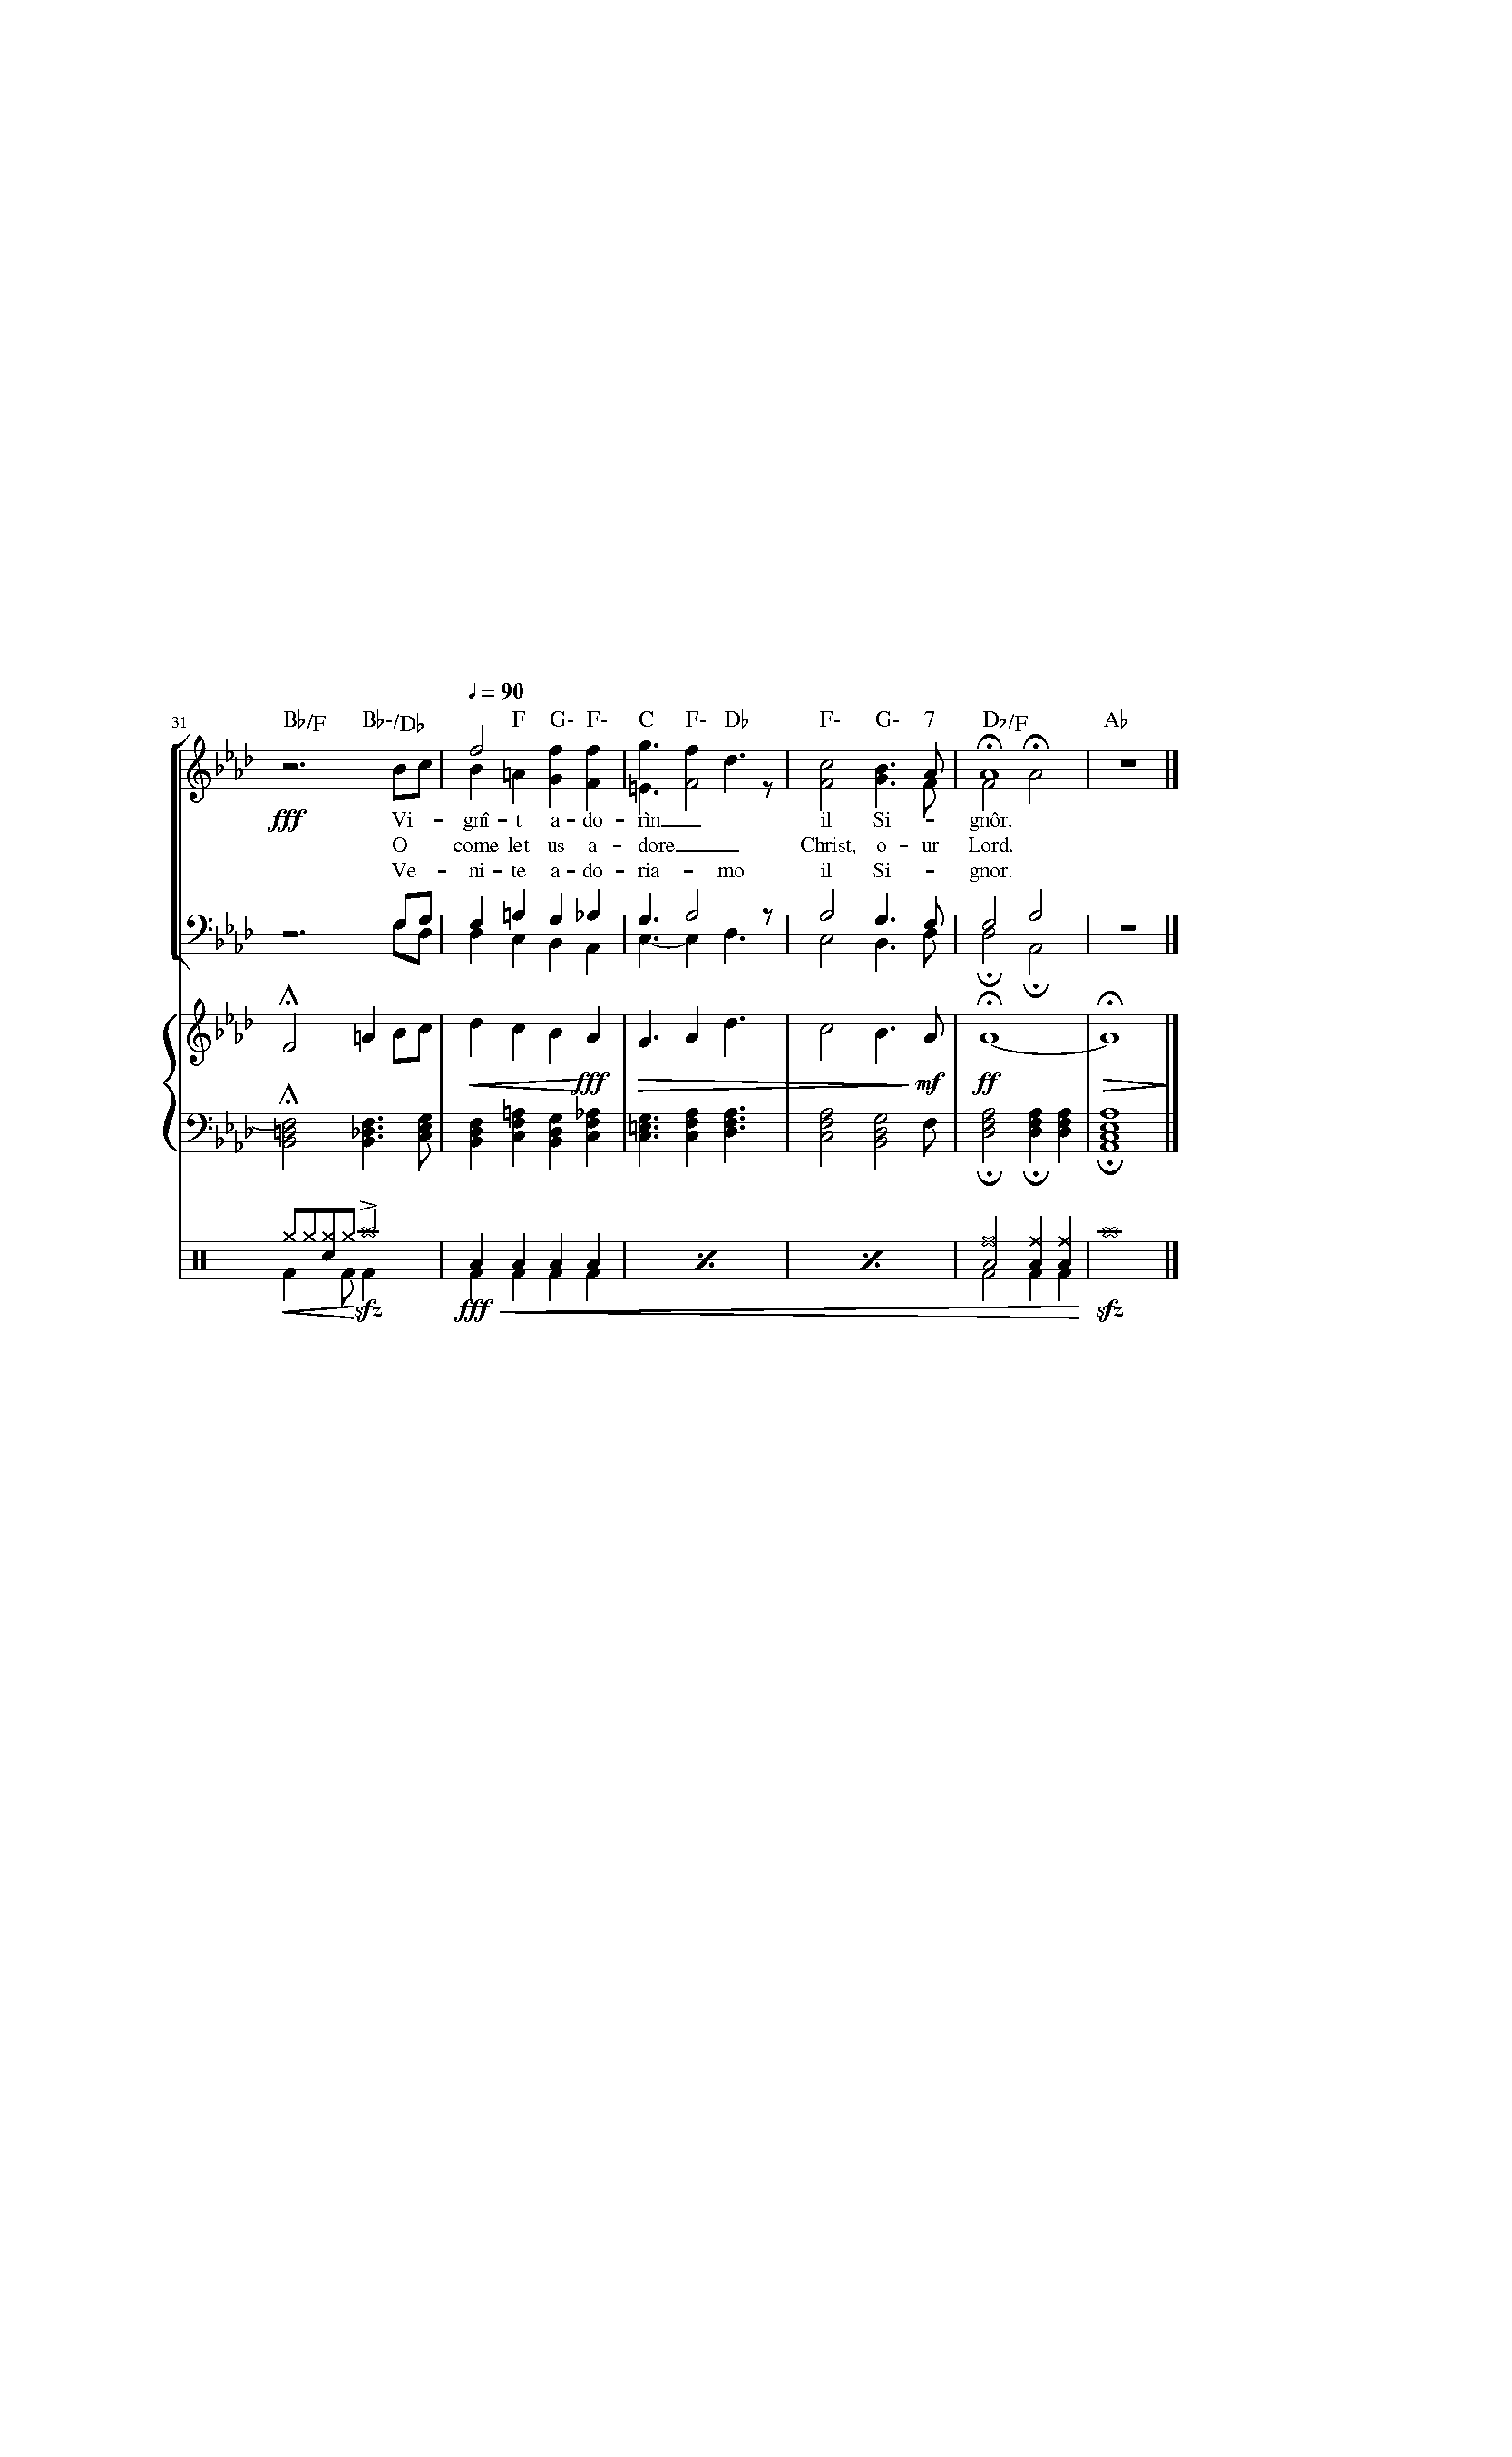
\includegraphics[width=\textwidth]{img/spartiti}
    \end{subfigure}
  \end{figure}
}
\only<5>{
  Presentazioni\\~\\
  \fbox{
\includegraphics[width=0.7\textwidth,page=1]{img/presentazione}}
}
\only<6>{
  Scrivere facilmente con più alfabeti\\~\\
  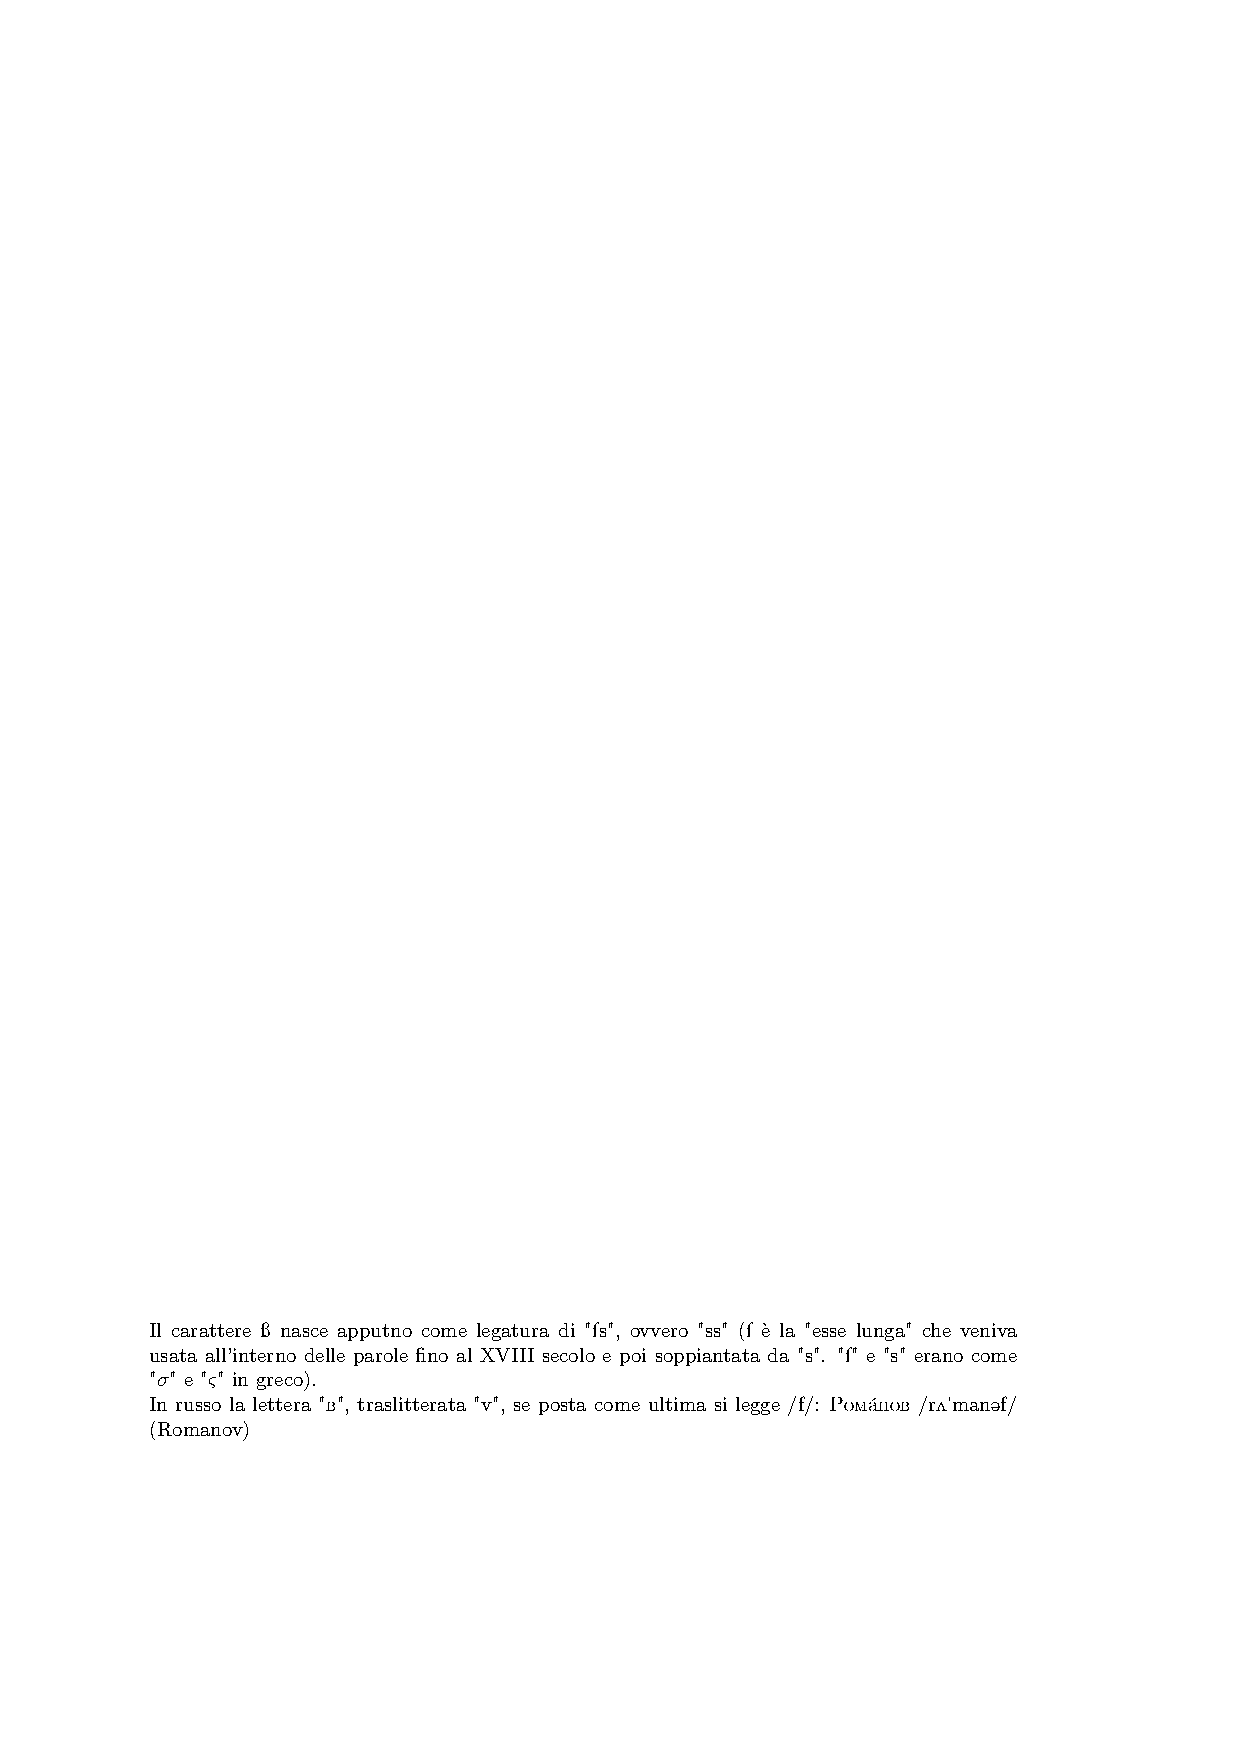
\includegraphics[width=\textwidth,page=1]{img/alfabeti}
}
}

\frame{\transfade\centering
\frametitle{Come si utilizza \LaTeX?}
\begin{itemize}
  \item<2->{Editor di testo + linea di comando}
  \item<3->{Editor avanzato (es: Miktex)}
\end{itemize}
}

\section{Primi passi}
\frame{\transfade\centering
\frametitle{Tipologie di documento}
\begin{itemize}
  \item<2-> \textbf{\emph{article}} per scrivere articoli (scientifici) senza capitoli
  \item<3-> \textbf{report} per scrivere relazioni o tesi suddivise in capitoli
  \item<4-> \textbf{letter} per scrivere lettere
  \item<5-> \textbf{\emph{book}} per scrivere libri
  \item<6-> {\footnotesize\textbf{memoir} per scrivere libri complessi}
  \item<7-> {\footnotesize\textbf{beamer} per presentazioni}
  \item<8-> \textbf{\dots}
  \end{itemize}
}

\begin{frame}[fragile]\transfade\centering
\frametitle{Esempio minimale (1/2)}
\begin{verbatim}
  \documentclass[a4paper, 12pt]{report}
    %    10pt, 11pt, 12 pt ↑      ↑ classe
    %    twocolumn dispone il testo su due colonne

  \pdfpagewidth\paperwidth      % per assicurarsi che nel pdf
  \pdfpageheight\paperheight    % sia riempita tutta la pagina

  \usepackage[italian]{babel}   % lingua usata nel documento
  \usepackage[utf8]{inputenc}  % se non va usare utf8x
  \usepackage[T1]{fontenc}
\end{verbatim}\dots\\~
\end{frame}
\begin{frame}[fragile]\transfade\centering
  \frametitle{Esempio minimale (2/2)}
  {\small~\\[-0.5cm]\dots\\[-0.5cm]\begin{verbatim}
    \begin{document}
      \title{Titolo del documento}\author{Autore}\date{Data}
      \maketitle

      \tableofcontents  %indice

      \chapter{Nome capitolo}
        \section{Nome sezione}
          \subsection{Nome sottosezione}
            \subsubsection{Nome sotto-sottosezione}
              testo

    \end{document}
  \end{verbatim}}
\end{frame}

\frame{\transfade\centering
\frametitle{Font}
\begin{itemize}
  \item<2->{\texttt{\textbf{\textbackslash textbf}}\{testo\} \textbf{grassetto}}
  \item<2->{\texttt{\textbf{\textbackslash emph}}\{testo\} \emph{italico} ("corsivo")}
  \item<2->{\texttt{\textbf{\textbackslash texttt}}\{testo\} \texttt{monospace}}
\end{itemize}
\begin{itemize}
  \item<3->{\{\texttt{\textbf{\textbackslash tiny}} testo \}}
  \item<3->{\{\texttt{\textbf{\textbackslash footnotesize}} testo \}}
  \item<3->{\{\texttt{\textbf{\textbackslash small}} testo \}}
  \item<3->{\{\texttt{\textbf{\textbackslash large}} testo \}}
  \item<3->{\{\texttt{\textbf{\textbackslash Large}} testo \}}
\end{itemize}
}

\frame{\transfade\centering
\frametitle{Ultimi dettagli}
\visible<2->{Andare a capo}
  \begin{itemize}
    \item<2->{\texttt{\textbf{\textbackslash\textbackslash}} a capo}
    \item<2->{\texttt{\textbf{\textbackslash par}} nuovo paragrafo}
  \end{itemize}
\visible<3->{Alcuni simboli}
  \begin{itemize}
    \item<3->{\texttt{\textbf{\textbackslash\$}} \$}
    \item<3->{\texttt{\textbf{\textbackslash\%}} \%}
    \item<3->{\texttt{\textbf{\textbackslash\_}} \_}
  \end{itemize}
}

\section{Matematica}
\begin{frame}[fragile]\transfade\centering
    Per le formule matemtiche e per altri simboli occorre includere i seguenti pacchetti (nel preambolo):
    \verb!\usepackage{amsmath,amssymb}!
\end{frame}
\frame{\transfade\centering
\frametitle{Formule in linea}
  \visible<2->{\texttt{Come tutti sanno \textbf{\$2\^{}2 = 4\$} e \textbf{\$2 \textbackslash times 2 = 4\$}}}\\
  \visible<3->{Come tutti sanno $2^2 = 4$ e $2 \times 2= 4$}
}
\frame{\transfade\centering
\frametitle{Formule in evidenza}
  \visible<2->{\texttt{Data la funzione: \textbf{\textbackslash[ f(x)= x\^{}2 + \textbackslash frac\{x\}\{2\} \textbackslash]}}}\\~\\
  \visible<3->{Data la funzione: \[ f(x)= x^2 + \frac{x}{2} \]}
}
\frame{\transfade\centering
\frametitle{Formule in evidenza numerate}
  \visible<2->{\texttt{Data la funzione: \textbf{\textbackslash begin\{equation\} f(x):= x\^{}2 + \textbackslash frac\{x\}\{2\} \only<4->{\textbackslash label\{eq:\emph{nomeFormula}\}} \textbackslash end\{equation\}}}}\\~\\
\visible<3->{Data la funzione: \begin{equation} f(x):= x^2 + \frac{x}{2} \label{eq:nomeFormula}\end{equation}}
  \visible<5->{\texttt{Vedi formula \textbf{\textbackslash ref\{eq:\emph{nomeFormula}\}}}}\\~\\
\visible<6->{Vedi formula \ref{eq:nomeFormula}}
}

\begin{frame}[fragile]\transfade\centering
  \verb!\forall x \in X, \quad \exists y \leq \epsilon!\\$\forall x \in X, \quad \exists y \leq \epsilon$\\~\\
  \verb!\cos (2\theta) = \cos^2 \theta - \sin^2 \theta!\\$\cos (2\theta) = \cos^2 \theta - \sin^2 \theta$\\~\\
  \verb!\lim_{x \to \infty} \exp(-x) = 0! ~~ $
  \lim_{x \to \infty} \exp(-x) = 0$\\~\\
  \verb!x \equiv a \pmod{b}! ~~ $x \equiv a \pmod{b}$\\~\\
  \verb!k_{n+1} = n^2 + k_n^2 - k_{n-1}!\\$k_{n+1} = n^2 + k_n^2 - k_{n-1}$\\~\\
  \verb!\sqrt{2} \sqrt[n]{\frac{a}{b}}! ~~ $\sqrt2$ ~ $\sqrt[n]{\frac{a}{b}}$\\~
\end{frame}
\begin{frame}[fragile]\transfade\centering
  \verb!\sum_{i=1}^{10} t_i! ~~ $\sum_{i=1}^{10} t_i$\\~\\
  \verb!\displaystyle\sum_{i=1}^{10} t_i! ~~ $\displaystyle\sum_{i=1}^{10} t_i$\\~\\
  \verb!\int_0^\infty \mathrm{e}^{-x}\,\mathrm{d}x! ~~ $\int_0^\infty \mathrm{e}^{-x}\,\mathrm{d}x$\\~\\
  \verb!A_{2,2} = \begin{pmatrix}         !\\
  \verb!              a_{1,1} & a_{1,2} \\!\\
  \verb!              a_{2,1} & a_{2,2}   !\\
  \verb!          \end{pmatrix}           !\\~\\
    $A_{2,2} = \begin{pmatrix}a_{1,1} & a_{1,2} \\a_{2,1} & a_{2,2}\end{pmatrix}$\\~
\end{frame}

\section{Elenchi}
\begin{frame}[fragile]\transfade\centering
  \frametitle{Elenchi numerati}
  \verb!\begin{enumerate}!\\
  \verb!  \item Tizio     !\\
  \verb!  \item Caio      !\\
  \verb!  \item Sempronio!\\
  \verb!\end{enumerate}  !\\~
  \only<2->{\begin{enumerate}\centering
    \item \texttt{Tizio~~~~~}
    \item \texttt{Caio~~~~~~}
    \item \texttt{Sempronio}
  \end{enumerate}}
\end{frame}
\begin{frame}[fragile]\transfade\centering
  \frametitle{Elenchi puntati}
  \verb!\begin{itemize}   !\\
  \verb!  \item Tizio     !\\
  \verb!  \item Caio      !\\
  \verb!  \item Sempronio!\\
  \verb!\end{itemize}     !\\~
  \only<2->{\begin{itemize}\centering
    \item \texttt{Tizio~~~~~}
    \item \texttt{Caio~~~~~~}
    \item \texttt{Sempronio}
  \end{itemize}}
\end{frame}
\begin{frame}[fragile]\transfade\centering
  \frametitle{Descrizioni}
  \verb!\begin{description}              !\\
  \verb!  \item[Responsabile] Tizio      !\\
  \verb!  \item[Supervisore] Caio        !\\
  \verb!  \item[Collaboratore] Sempronio!\\
  \verb!\end{description}                !\\~
  \only<2->{\begin{description}\centering
    \item[\texttt{Responsabile~}] \texttt{Tizio~~~~~}
    \item[\texttt{Supervisore~~}] \texttt{Caio~~~~~~}
    \item[\texttt{Collaboratore}] \texttt{Sempronio}
  \end{description}}
\end{frame}

\section{Note}
\begin{frame}[fragile]\transfade\centering
  \frametitle{Note a piè di pagina}
  \verb!Questo è un testo\footnote{è un testo molto corto} di prova!\\~\\
  \only<2->{Questo è un testo\footnote{è un testo molto corto} di prova}~\\~
\end{frame}
\begin{frame}\transfade\centering
  \frametitle{Note al margine}
  \begin{columns}
    \column{.1\textwidth}
      \only<2->{~\\[5px]$A = l^2$}
    \column{.9\textwidth}
      \texttt{L'area\textbackslash marginpar\{\$A = l\^{}2\$\} del quadrato vale 5}\\~\\
      \only<2->{L'area del quadrato vale 5}~\\~
  \end{columns}
\end{frame}


\setbeamercolor{background canvas}{bg=black}
\frame[plain]{\transfade}

\end{document}
